\documentclass{IEEEtran}
\usepackage{cite}
\usepackage{amsmath,amssymb,amsfonts}
\usepackage{algorithmic}
\usepackage{graphicx}
\usepackage{textcomp}

% Disable all paragraph indentation
\setlength{\parindent}{0pt}

\def\BibTeX{{\rm B\kern-.05em{\sc i\kern-.025em b}\kern-.08em
    T\kern-.1667em\lower.7ex\hbox{E}\kern-.125emX}}
\begin{document}
\title{Flu Shot Learning: \\Predicting H1N1 and Seasonal Flu Vaccination}
\author{Jorge Pais, José Baptista and Pedro Duarte\\ 
    \textit{up201904841@edu.fe.up.pt; up201904814@edu.fe.up.pt; up201905050@edu.fe.up.pt}}

\maketitle

\begin{abstract}
    The model used in this study was a gradient boosting classifier, which was evaluated on separate test data provided by the NHFS using the area under the Receiver Operating Characteristic (ROC) curve as a performance metric. After necessary parameter tuning, the model was able to achieve a score of 0.8415.
\end{abstract}

\section{Introduction}
Pandemics have rarely taken center stage in the way they have recently with COVID-19 in 2020.  Vaccines are a key public health measure used to fight infectious diseases like COVID-19. They provide immunization for individuals, and enough immunization in a community can further reduce the spread of diseases through "herd immunity."
We will look at a recent historical pandemic, also of a highly infectious respiratory disease: the 2009 H1N1 influenza pandemic.

In 2009, the H1N1 influenza virus, also known as swine flu, caused a global pandemic that was estimated to have resulted in 150,000 to 600,000 deaths worldwide. A vaccine for H1N1 became available in October of that year. In this study, we developed a machine learning model to help estimate the probability of a person receiving seasonal and H1N1 vaccines. 

\textit{Dar alguma contextualizacao do que é que vai ser construido neste trabalho}

\section{Data Set Analysis / Data Resources}

\subsection{DataSet}
In this research work, the dataset used was provided by DrivenData, and it comes from the National 2009 H1N1 Flu Survey (NHFS) which included 36 attributes and was collected through telephone interviews. The dataset consists of 36 columns (attributes) of which respondent id is unique and 35 other columns out of which most of them were binary type and others were of ordinal type. The goal was to predict the probability of a person receiving seasonal and H1N1 vaccines. The predicted values were later evaluated based on the ROC curve. The problem falls under multilabel problem, not a multiclass problem.

\subsection{Data Cleaning and Pre-processing}
The first step in the data analysis was to check if the data has any duplicate and missing values, duplicates were not observed, but the dataset had many missing values in different attributes ranging from 19 to 13470. So, our first concern was to clean the data. Since the attributes employment concern and employment occupation had the highest missing data (13470 values) we decided to drop the same along with respondent id as it was of no use. The next step involved checking of correlation  between the attributes. This was done using the seaborn library’s correlation heatmap. It was noted that two attributes named doctor recc H1N1 vaccine and doctor recc seasonal vaccine attributes were positively correlated by 60\%.

Hence, only one attribute has been retained. In the next step, the missing data were handled. Two different imputation methods are implemented in this project, the first one being median imputation and the second one, the one-hot encoder. The algorithms and packages used in this work require numeric data, and not categorical data. Therefore, a unique numerical value is assigned to each category in the object columns. This method can cause problems, as the model might not recognize the data as categorical and would process it on a scale. This leads to incorrect weight assignments. To avoid this problem, one-hot encoder is used, which encodes a category in a 1-hot vector, where the position in the vector refers to each category and its size is equal to the number of categories. Simple imputer is used to fill in missing data using median method. The Pandas library in Python identifies missing values as NaN. After the data is cleaned and pre-processed, graphical visualizations are generated.
\begin{center}
    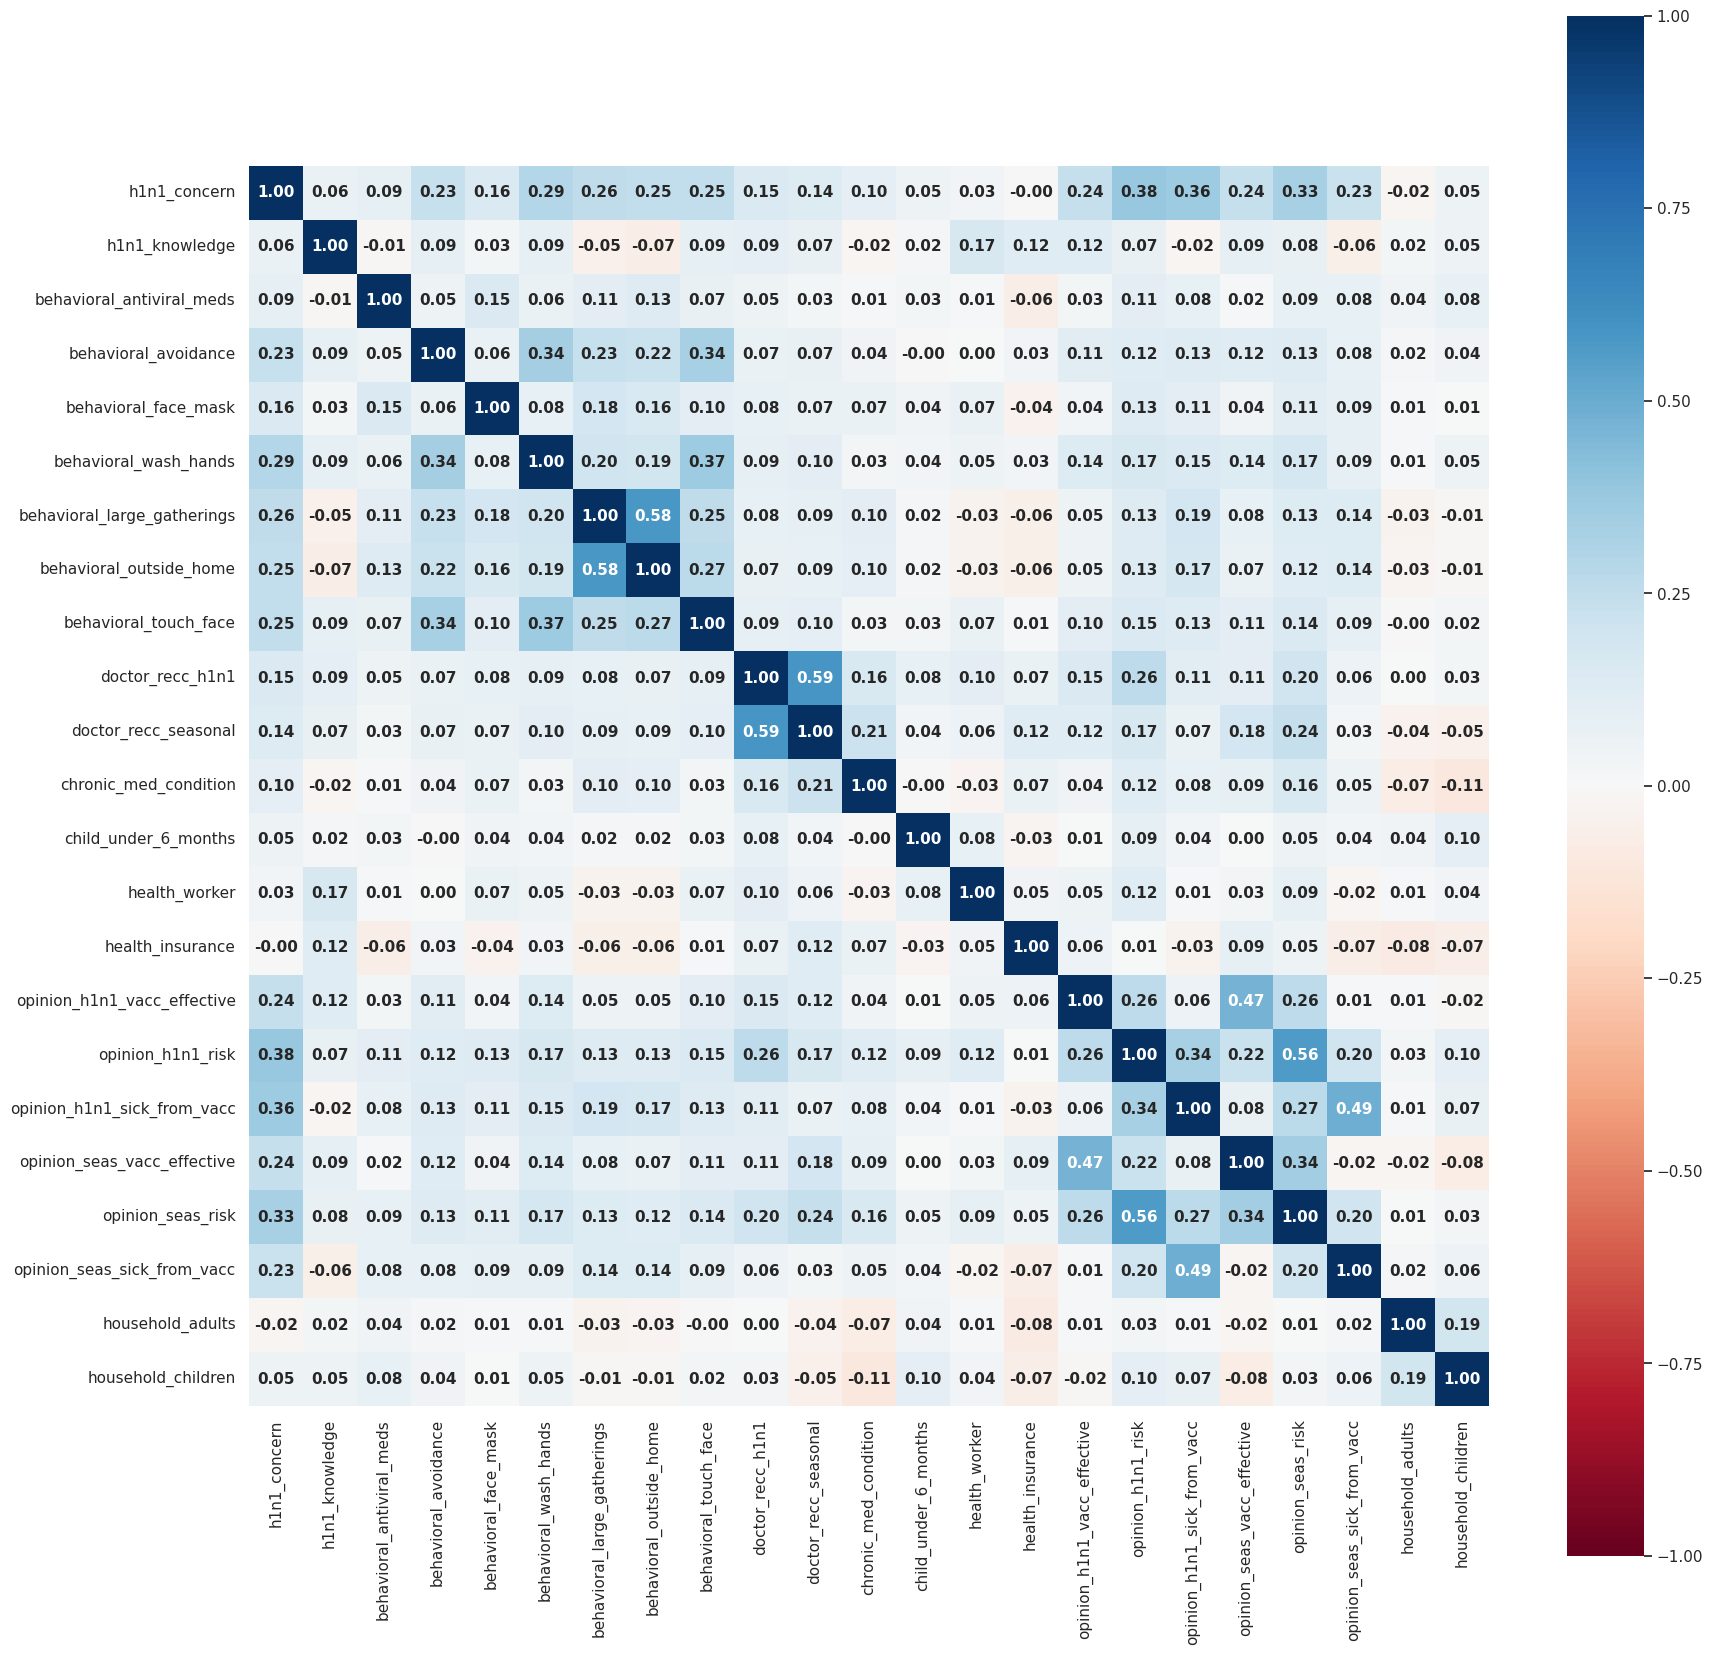
\includegraphics[width = 8cm,height=8cm]{figures/Heatmap.png}\\  Figure 1 - Feature Correlation Heatmap
\end{center}

\subsection{Class Balance}

\section{Performance Metric}

\textit{Explicar aqui o que é o ROC}

\section{Model Pipeline}

\textit{Talvez seja melhor condensar esta secção com a proxima, sob metodologia}

\textit{Meter aqui aquelas figuras do model pipeline, e mostrar o esquema lógico do que vai ser construido}

\begin{center}
    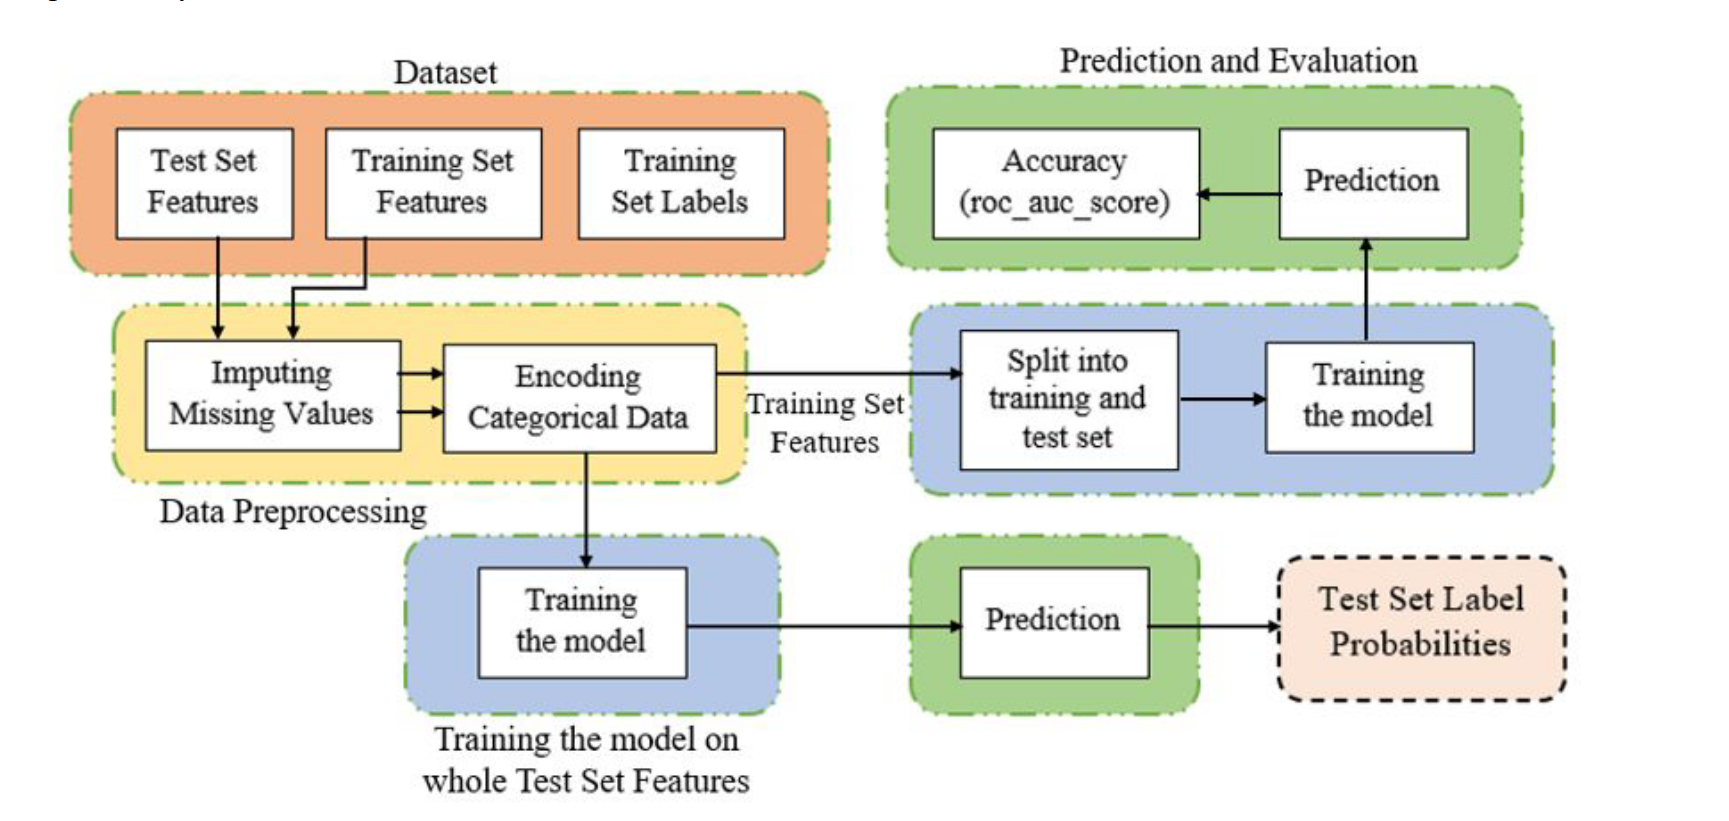
\includegraphics[width = 5cm]{figures/ModelPipeline.png}\\
    Figure 3.x.x - Model pipeline example
\end{center}

\section{Models}

\textit{Meter aqui todos os modelos que foram experimentados}

\section{Results}

\section{Conclusion}

\vfill
\pagebreak

\section{Reference Examples}

\begin{itemize}

\item \emph{Basic format for books:}\\
J. K. Author, ``Title of chapter in the book,'' in \emph{Title of His Published Book, x}th ed. City of Publisher, (only U.S. State), Country: Abbrev. of Publisher, year, ch. $x$, sec. $x$, pp. \emph{xxx--xxx.}\\
See \cite{b1,b2}.

\item \emph{Basic format for periodicals:}\\
J. K. Author, ``Name of brief,'' \emph{Abbrev. Title of Periodical}, vol. \emph{x, no}. $x, $pp\emph{. xxx--xxx, }Abbrev. Month, year, DOI. 10.1109.\emph{XXX}.123456.\\
See \cite{b3}--\cite{b5}.

\item \emph{Basic format for reports:}\\
J. K. Author, ``Title of report,'' Abbrev. Name of Co., City of Co., Abbrev. State, Country, Rep. \emph{xxx}, year.\\
See \cite{b6,b7}.

\item \emph{Basic format for handbooks:}\\
\emph{Name of Manual/Handbook, x} ed., Abbrev. Name of Co., City of Co., Abbrev. State, Country, year, pp. \emph{xxx--xxx.}\\
See \cite{b8,b9}.

\item \emph{Basic format for books (when available online):}\\
J. K. Author, ``Title of chapter in the book,'' in \emph{Title of
Published Book}, $x$th ed. City of Publisher, State, Country: Abbrev.
of Publisher, year, ch. $x$, sec. $x$, pp. \emph{xxx--xxx}. [Online].
Available: \underline{http://www.web.com}\\
See \cite{b10}--\cite{b13}.

\item \emph{Basic format for journals (when available online):}\\
J. K. Author, ``Name of brief,'' \emph{Abbrev. Title of Periodical}, vol. $x$, no. $x$, pp. \emph{xxx--xxx}, Abbrev. Month, year. Accessed on: Month, Day, year, DOI: 10.1109.\emph{XXX}.123456, [Online].\\
See \cite{b14}--\cite{b16}.

\item \emph{Basic format for briefs presented at conferences (when available online): }\\
J.K. Author. (year, month). Title. presented at abbrev. conference title. [Type of Medium]. Available: site/path/file\\
See \cite{b17}.

\item \emph{Basic format for reports and handbooks (when available online):}\\
J. K. Author. ``Title of report,'' Company. City, State, Country. Rep. no., (optional: vol./issue), Date. [Online] Available: site/path/file\\
See \cite{b18,b19}.

\item \emph{Basic format for computer programs and electronic documents (when available online): }\\
Legislative body. Number of Congress, Session. (year, month day). \emph{Number of bill or resolution}, \emph{Title}. [Type of medium]. Available: site/path/file\\
\textbf{\emph{NOTE: }ISO recommends that capitalization follow the accepted practice for the language or script in which the information is given.}\\
See \cite{b20}.

\item \emph{Basic format for patents (when available online):}\\
Name of the invention, by inventor's name. (year, month day). Patent Number [Type of medium]. Available: site/path/file\\
See \cite{b21}.

\item \emph{Basic format}\emph{for conference proceedings (published):}\\
J. K. Author, ``Title of brief,'' in \emph{Abbreviated Name of Conf.}, City of Conf., Abbrev. State (if given), Country, year, pp. \emph{xxxxxx.}\\
See \cite{b22}.

\item \emph{Example for briefs presented at conferences (unpublished):}\\
See \cite{b23}.

\item \emph{Basic format for patents}$:$\\
J. K. Author, ``Title of patent,'' U.S. Patent \emph{x xxx xxx}, Abbrev. Month, day, year.\\
See \cite{b24}.

\item \emph{Basic format for theses (M.S.) and dissertations (Ph.D.):}
\begin{enumerate}
\item J. K. Author, ``Title of thesis,'' M.S. thesis, Abbrev. Dept., Abbrev. Univ., City of Univ., Abbrev. State, year.
\item J. K. Author, ``Title of dissertation,'' Ph.D. dissertation, Abbrev. Dept., Abbrev. Univ., City of Univ., Abbrev. State, year.
\end{enumerate}
See \cite{b25,b26}.

\item \emph{Basic format for the most common types of unpublished references:}
\begin{enumerate}
\item J. K. Author, private communication, Abbrev. Month, year.
\item J. K. Author, ``Title of brief,'' unpublished.
\item J. K. Author, ``Title of brief,'' to be published.
\end{enumerate}
See \cite{b27}--\cite{b29}.

\item \emph{Basic formats for standards:}
\begin{enumerate}
\item \emph{Title of Standard}, Standard number, date.
\item \emph{Title of Standard}, Standard number, Corporate author, location, date.
\end{enumerate}
See \cite{b30,b31}.

\item \emph{Article number in~reference examples:}\\
See \cite{b32,b33}.

\item \emph{Example when using et al.:}\\
See \cite{b34}.

\end{itemize}

\begin{thebibliography}{00}

\bibitem{b1} G. O. Young, ``Synthetic structure of industrial plastics,'' in \emph{Plastics,} 2\textsuperscript{nd} ed., vol. 3, J. Peters, Ed. New York, NY, USA: McGraw-Hill, 1964, pp. 15--64.

\bibitem{b2} W.-K. Chen, \emph{Linear Networks and Systems.} Belmont, CA, USA: Wadsworth, 1993, pp. 123--135.

\bibitem{b3} J. U. Duncombe, ``Infrared navigation---Part I: An assessment of feasibility,'' \emph{IEEE Trans. Electron Devices}, vol. ED-11, no. 1, pp. 34--39, Jan. 1959, 10.1109/TED.2016.2628402.

\bibitem{b4} E. P. Wigner, ``Theory of traveling-wave optical laser,'' \emph{Phys. Rev}., vol. 134, pp. A635--A646, Dec. 1965.

\bibitem{b5} E. H. Miller, ``A note on reflector arrays,'' \emph{IEEE Trans. Antennas Propagat}., to be published.

\bibitem{b6} E. E. Reber, R. L. Michell, and C. J. Carter, ``Oxygen absorption in the earth's atmosphere,'' Aerospace Corp., Los Angeles, CA, USA, Tech. Rep. TR-0200 (4230-46)-3, Nov. 1988.

\bibitem{b7} J. H. Davis and J. R. Cogdell, ``Calibration program for the 16-foot antenna,'' Elect. Eng. Res. Lab., Univ. Texas, Austin, TX, USA, Tech. Memo. NGL-006-69-3, Nov. 15, 1987.

\bibitem{b8} \emph{Transmission Systems for Communications}, 3\textsuperscript{rd} ed., Western Electric Co., Winston-Salem, NC, USA, 1985, pp. 44--60.

\bibitem{b9} \emph{Motorola Semiconductor Data Manual}, Motorola Semiconductor Products Inc., Phoenix, AZ, USA, 1989.

\bibitem{b10} G. O. Young, ``Synthetic structure of industrial
plastics,'' in Plastics, vol. 3, Polymers of Hexadromicon, J. Peters,
Ed., 2\textsuperscript{nd} ed. New York, NY, USA: McGraw-Hill, 1964, pp. 15-64.
[Online]. Available:
\underline{http://www.bookref.com}.

\bibitem{b11} \emph{The Founders' Constitution}, Philip B. Kurland
and Ralph Lerner, eds., Chicago, IL, USA: Univ. Chicago Press, 1987.
[Online]. Available: \underline{http://press-pubs.uchicago.edu/founders/}

\bibitem{b12} The Terahertz Wave eBook. ZOmega Terahertz Corp., 2014.
[Online]. Available:
\underline{http://dl.z-thz.com/eBook/zomega\_ebook\_pdf\_1206\_sr.pdf}. Accessed on: May 19, 2014.

\bibitem{b13} Philip B. Kurland and Ralph Lerner, eds., \emph{The
Founders' Constitution.} Chicago, IL, USA: Univ. of Chicago Press,
1987, Accessed on: Feb. 28, 2010, [Online] Available:
\underline{http://press-pubs.uchicago.edu/founders/}

\bibitem{b14} J. S. Turner, ``New directions in communications,'' \emph{IEEE J. Sel. Areas Commun}., vol. 13, no. 1, pp. 11-23, Jan. 1995.

\bibitem{b15} W. P. Risk, G. S. Kino, and H. J. Shaw, ``Fiber-optic frequency shifter using a surface acoustic wave incident at an oblique angle,'' \emph{Opt. Lett.}, vol. 11, no. 2, pp. 115--117, Feb. 1986.

\bibitem{b16} P. Kopyt \emph{et al., ``}Electric properties of graphene-based conductive layers from DC up to terahertz range,'' \emph{IEEE THz Sci. Technol.,} to be published. DOI: 10.1109/TTHZ.2016.2544142.

\bibitem{b17} PROCESS Corporation, Boston, MA, USA. Intranets:
Internet technologies deployed behind the firewall for corporate
productivity. Presented at INET96 Annual Meeting. [Online].
Available: \underline{http://home.process.com/Intranets/wp2.htp}

\bibitem{b18} R. J. Hijmans and J. van Etten, ``Raster: Geographic analysis and modeling with raster data,'' R Package Version 2.0-12, Jan. 12, 2012. [Online]. Available: \underline {http://CRAN.R-project.org/package=raster} 

\bibitem{b19} Teralyzer. Lytera UG, Kirchhain, Germany [Online].
Available:
\underline{http://www.lytera.de/Terahertz\_THz\_Spectroscopy.php?id=home}, Accessed on: Jun. 5, 2014

\bibitem{b20} U.S. House. 102\textsuperscript{nd} Congress, 1\textsuperscript{st} Session. (1991, Jan. 11). \emph{H. Con. Res. 1, Sense of the Congress on Approval of}  \emph{Military Action}. [Online]. Available: LEXIS Library: GENFED File: BILLS

\bibitem{b21} Musical toothbrush with mirror, by L.M.R. Brooks. (1992, May 19). Patent D 326 189 [Online]. Available: NEXIS Library: LEXPAT File: DES

\bibitem{b22} D. B. Payne and J. R. Stern, ``Wavelength-switched pas- sively coupled single-mode optical network,'' in \emph{Proc. IOOC-ECOC,} Boston, MA, USA, 1985, pp. 585--590.

\bibitem{b23} D. Ebehard and E. Voges, ``Digital single sideband detection for interferometric sensors,'' presented at the \emph{2\textsuperscript{nd} Int. Conf. Optical Fiber Sensors,} Stuttgart, Germany, Jan. 2-5, 1984.

\bibitem{b24} G. Brandli and M. Dick, ``Alternating current fed power supply,'' U.S. Patent 4 084 217, Nov. 4, 1978.

\bibitem{b25} J. O. Williams, ``Narrow-band analyzer,'' Ph.D. dissertation, Dept. Elect. Eng., Harvard Univ., Cambridge, MA, USA, 1993.

\bibitem{b26} N. Kawasaki, ``Parametric study of thermal and chemical nonequilibrium nozzle flow,'' M.S. thesis, Dept. Electron. Eng., Osaka Univ., Osaka, Japan, 1993.

\bibitem{b27} A. Harrison, private communication, May 1995.

\bibitem{b28} B. Smith, ``An approach to graphs of linear forms,'' unpublished.

\bibitem{b29} A. Brahms, ``Representation error for real numbers in binary computer arithmetic,'' IEEE Computer Group Repository, Brief R-67-85.

\bibitem{b30} IEEE Criteria for Class IE Electric Systems, IEEE Standard 308, 1969.

\bibitem{b31} Letter Symbols for Quantities, ANSI Standard Y10.5-1968.

\bibitem{b32} R. Fardel, M. Nagel, F. Nuesch, T. Lippert, and A. Wokaun, ``Fabrication of organic light emitting diode pixels by laser-assisted forward transfer,'' \emph{Appl. Phys. Lett.}, vol. 91, no. 6, Aug. 2007, Art. no. 061103.~

\bibitem{b33} J. Zhang and N. Tansu, ``Optical gain and laser characteristics of InGaN quantum wells on ternary InGaN substrates,'' \emph{IEEE Photon. J.}, vol. 5, no. 2, Apr. 2013, Art. no. 2600111

\bibitem{b34} S. Azodolmolky~\emph{et al.}, Experimental demonstration of an impairment aware network planning and operation tool for transparent/translucent optical networks,''~\emph{J. Lightw. Technol.}, vol. 29, no. 4, pp. 439--448, Sep. 2011.

\end{thebibliography}

\end{document}
